\documentclass[12pt]{extarticle}
\usepackage{tempora}
\usepackage[T1, T2A]{fontenc}
\usepackage[utf8]{inputenc}
\usepackage[english, ukrainian]{babel}
\usepackage{geometry}
\usepackage{graphicx}
\usepackage{multirow}
\usepackage{multicol}
\usepackage{float}
\graphicspath{{/home/artem/Pictures}}
\geometry
{
    a4paper,
    left=30mm,
    top=15mm,
    right=20mm,
    bottom=15mm,
}

\begin{document}
\begin{titlepage}
    \begin{center}
        \textbf{\normalsize{\MakeUppercase{
            Міністерство Освіти і науки України
            Національний університет "Львівська політехніка"
        }}}

        \begin{flushright}
        \textbf{ІКНІ}\\
        Кафедра \textbf{ПЗ}
        \end{flushright}
        \vspace{15mm}

        \includegraphics[width=0.4\textwidth]{lpnu_logo.png}

        \vspace*{\fill}

        \textbf{\normalsize{\MakeUppercase{Звіт}}}
            
        До лабораторної роботи №6

        \textbf{на тему:} “Виведення на монітор тексту і графіки”

        \textbf{з дисципліни:} “Архітектура комп’ютера”
            
        \vspace*{\fill}

        \begin{flushright}

            \textbf{Лектор:}\\
            доцент кафедри ПЗ\\
            Крук О.Г.\\
            \vspace{12pt}

            \textbf{Виконав:}\\
            студент групи ПЗ-24\\
            Губик А. С.\\
            \vspace{12pt}

            \textbf{Прийняв:}\\
            доцент кафедри ПЗ\\
            Задорожний І. М.\\
        \vspace{12pt}
        \end{flushright}

        Львів -- 2023
            
            
    \end{center}
\end{titlepage}

\textbf{Тема роботи:}Виведення на монітор тексту і графіки

\vspace{12pt}

\textbf{Мета роботи:} опанувати функції BIOS для роботи з відео в текстовому
та графічному режимах; розвинути навики складання програм для виведення
різнокольорових рядків символів та графічних зображень; відтранслювати і
виконати в режимі відлагодження програми, складені відповідно до свого
варіанту.

\subsection*{Індивідуальне завдання}
\begin{enumerate}
\item Опишіть рядки символів, в яких вкажіть прізвище, ім’я, по батькові.
\item Сформуйте байти атрибутів (різні) для кожного символу в кожному
рядку символів.
\item Очистіть екран.
\item В текстовому режимі початковий номер рядка на екрані визначається як
остача від ділення номера в списку групи на 10 (в звіті наведіть розрахунок всіх
номерів рядків і стовпців, довжин сторін, кольору тощо).
\item Початковий номер стовпця на екрані визначається як сума номера групи
і номера в списку групи.
\item Шляхом безпосереднього записування тексту в першу сторінку
текстової відеопам'яті виведіть рядок символів з прізвищем у початковий рядок,
починаючи з початкового стовпця (функцій MS DOS не використовувати!).
\item Рядок символів з іменем виведіть в рядок, номер якого дорівнює
початковому+2, починаючи з стовпця, номер якого дорівнює початковому+3.
\item Рядок символів з по батькові виведіть в рядок, номер якого дорівнює
початковому+6, починаючи з стовпця, номер якого дорівнює початковому+8.
\item Зробіть копію екрану.
\item В графічному режимі 13h побудуйте прямокутник, ліва верхня вершина
якого розміщується в рядку, номер якого дорівнює кількості літер у прізвищі, і в
стовпці, номер якого дорівнює кількості літер в по батькові. Довжина
горизонтальної сторони прямокутника дорівнює потроєному номеру
групи+номер в списку групи. Довжина вертикальної сторони прямокутника
дорівнює подвоєному номеру групи+номер в списку групи. Колір прямокутника
виберіть за остачею від ділення номера групи на 3: 0 – червоний; 1 – зелений; 2
– синій.
\item Перевірте результат роботи програми.
\item Зробіть копію екрану.
\item У звіті наведіть текст програми
\end{enumerate}

\subsection*{Теоретичні відомості}
У текстовому режимі прикладна програма може вивести інформацію на
екран одним з таких способів.
• За допомогою функцій MS DOS. Якщо на комп'ютері встановлена
система MS DOS або її емулятор, для виведення текстових даних на екран можна
скористатися функціями переривання INT 21h. Дані функції дозволяють
перенаправити потоки введення-виведення на будь-який інший пристрій, такий
як принтер або диск. Виведення на екран за допомогою функцій переривання
INT 21h виконується досить повільно, і колір символів змінити не можна.
• За допомогою функцій BIOS. Вивести символи на екран можна також за
допомогою функцій переривання INT 10h, оброблення якого виконується
системою BIOS, а не DOS. Вони виконуються набагато швидше, ніж функції
переривання INT 21h, і дозволяють змінити колір тексту на екрані. При
заповненні символами великих областей на екрані за допомогою функцій
переривання INT 10h, можна помітити невелику затримку виведення. Крім того,
дані, що виводяться на екран, не можна перенаправити на інший пристрій.
• Прямий доступ в відеопам'ять. Вивести символи на екран можна також
шляхом переміщення їх безпосередньо в область пам'яті відеоадаптера. При
цьому досягається максимальна швидкість виведення, проте дані також можна
перенаправити на інший пристрій. На зорі розвитку ПК, коли основною
операційною системою була MS DOS, в прикладних програмах, таких як текстові
процесори і електронні таблиці, використовувався саме цей метод виведення
даних на екран. Слід зазначити, що даний метод також можна використовувати
при роботі програми в повноекранному режимі під керуванням операційних
систем Windows NT, 2000 і ХР.
Залежно від поставлених завдань, в застосунку може використовуватися
один з трьох запропонованих вище способів виведення даних на екран. Якщо на
перше місце ставиться швидкість виведення на екран, то потрібно скористатися
прямим виведенням у відеопам'ять. В інших випадках слід віддати перевагу
функціям BIOS. Функціями DOS варто користуватися тільки тоді, коли вихідний
потік даних може бути перенаправлений на інший пристрій або коли екран
спільно використовується кількома програмами. Слід зазначити, що для
виведення даних на екран у функціях MS DOS використовуються функції BIOS,
а у функціях BIOS - прямий доступ до відеопам'яті.
Запуск програм в повноекранному режимі
Програми, в яких використовуються відеофункції BIOS, можуть
виконуватися в перерахованих нижче операційних системах і оболонках:
• "чистій" системі MS DOS;
• емуляторі DOS системи Linux;
• в повноекранному режимі в системі Windows.
У середовищі Windows в повноекранний режим можна перейти такими
способами.
• Спочатку створити ярлик для виконуваного ЕХЕ-файлу програми. Потім
відкрити вікно властивостей ярлика, перейти на вкладку Screen (Екран) і
встановити перемикач Full-screen mode (Повноекранний режим). Після цього
запустити програму за допомогою ярлика.
• Відкрити вікно командного рядка з меню Start (Пуск) і для перемикання
в повноекранний режим натиснути клавіші <Alt + Enter>. Потім за допомогою
команди CD (Change Directory - Змінити каталог) перейти в каталог, що містить
ЕХЕ-файл програми, і запустити програму з командного рядка, ввівши її ім'я і
натиснувши клавішу <Enter>. Якщо знову натиснути клавіші <Alt + Enter>, вікно
командного рядка перемикнеться з повноекранного у віконний режим.


\subsection*{Хід роботи}

\paragraph{1.}Програма що виводить П.І.Б.

\begin{verbatim}
    .model flat
    .stack 100h
    
    .data
    lastName	db "Artem"
    lastNameLen	dw $-lastName
    firstName	db "Hubyk"
    nameLen		dw $-firstName
    paternal	db "Serhiiovych"
    paternalLen dw $-paternal
    
    color db (0000 SHL 0) OR 0100
    
    .code
    
    
    
    
    
    main PROC
    
    int 10h;
    mov ax, @data 
    mov ds, ax 
    
    mov dl, 7 ; Початковий стовпець 
    mov dh, 3		; Початковий рядок
    mov ah, 02h				;   Встановимо положення курсора
    int 10h;
    
    mov cx, lastNameLen
    lea si, lastName
    L1:
    push cx				    ;   Збережемо лічильник циклу
    mov ah, 09h				;   Вивести символ і байт атрибутів
    mov al, [si]			;   Завантажимо символ, що виводиться
    mov bh, 0h				;   Відеосторінка 0
    mov bl, color			;   Байт атрибутів
    
    mov cx, 1d				;   Виведемо один символ
    int 10h
    
    inc dl					;   Збільшимо на 1 значення стовпця
    mov ah, 02h				;   Встановимо положення курсора
    int 10h
    
    add color,17			;   Значення наступного атрибута кольору
    inc si					;   Адреса наступного символу
    pop cx
    loop L1
    
    
    
    mov dl, 10 ; Початковий стовпець 
    mov dh, 5		; Початковий рядок
    mov ah, 02h				;   Встановимо положення курсора
    int 10h;
    
    mov cx, nameLen
    lea si, firstName
    L2:
    push cx				    ;   Збережемо лічильник циклу
    mov ah, 09h				;   Вивести символ і байт атрибутів
    mov al, [si]			;   Завантажимо символ, що виводиться
    mov bh, 0h				;   Відеосторінка 0
    mov bl, color			;   Байт атрибутів
    
    mov cx, 1d				;   Виведемо один символ
    int 10h
    
    inc dl					;   Збільшимо на 1 значення стовпця
    mov ah, 02h				;   Встановимо положення курсора
    int 10h
    
    add color,17			;   Значення наступного атрибута кольору
    inc si					;   Адреса наступного символу
    pop cx
    loop L2
    
    
    
    mov dl, 15 ; Початковий стовпець 
    mov dh, 9		; Початковий рядок
    
    
    mov ah, 02h				;   Встановимо положення курсора
    int 10h;
    
    mov cx, paternalLen
    lea si, paternal
    L3:
    push cx				    ;   Збережемо лічильник циклу
    mov ah, 09h				;   Вивести символ і байт атрибутів
    mov al, [si]			;   Завантажимо символ, що виводиться
    mov bh, 0h				;   Відеосторінка 0
    mov bl, color			;   Байт атрибутів
    
    mov cx, 1d				;   Виведемо один символ
    int 10h
    
    inc dl					;   Збільшимо на 1 значення стовпця
    mov ah, 02h				;   Встановимо положення курсора
    int 10h
    
    add color,17			;   Значення наступного атрибута кольору
    inc si					;   Адреса наступного символу
    pop cx
    loop L3
    
    
    
    
    
    
    int 10h
    
    mov ah, 4ch
    int 21h
    ;call CrLf 
    main ENDP
    
    
    END main
    

\end{verbatim}

\vspace{12pt}
\begin{figure}[H]
    \centering
    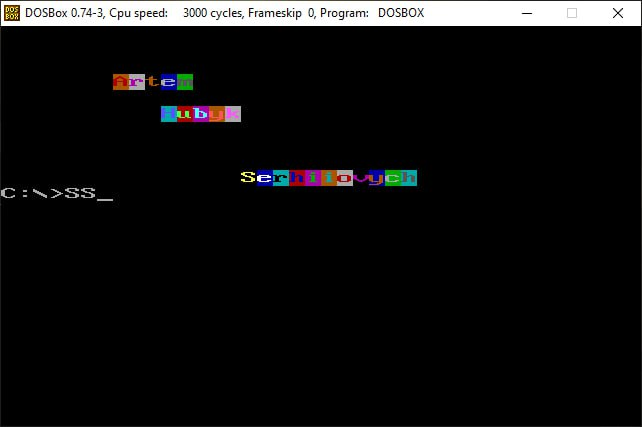
\includegraphics[width=0.90\textwidth]{name.jpg}
    \caption{}
\end{figure}

\paragraph{2.}Програма що малює прямокутник
\begin{verbatim}
.model flat
.stack 100h

.code

main proc
;int 10h

	mov ah, 0			; Встановимо новий відеорежим
	mov al, 13h			; номер 13h
	int 10h
	
	;розміри одного символа в рядку 8x8, для переміщення на відповідні позиції значення потрібно помножити на 8
	mov cx,80
	mov dx,40
	
	top:
	mov al,0100b
	mov ah,0ch
	int 10h
	inc cx
	mov ax, cx
	
	cmp ax, 80+75
		jne top
		
	mov cx,80
	mov dx,40 
	
	left:
		mov al,0100b
	mov ah,0ch
	int 10h
	inc dx
	mov ax, dx
	
	cmp ax, 40+51
		jne left
		
	mov cx,80 + 75
	mov dx,40  
	
	right:
		mov al,0100b
	mov ah,0ch
	int 10h
	inc dx
	mov ax, dx
	
	cmp ax, 40 + 51
		jne right	
	
	
	mov cx,80 
	mov dx, 51+32  
	
		
	mov cx,80 
	mov dx,51 + 40
	
	bottom:
	mov al,0100b
	mov ah,0ch
	int 10h
	inc cx
	mov ax, cx
	
	cmp ax, 80 + 75
		jne bottom
	
	
	
		
	;inc dx
	;mov cx,80
	;cmp dx, 119
	;	jne paint
	
	int 10h
	mov ah, 4ch
	int 21h
	
	main endp
end main

\end{verbatim}
\begin{figure}[H]
    \centering
    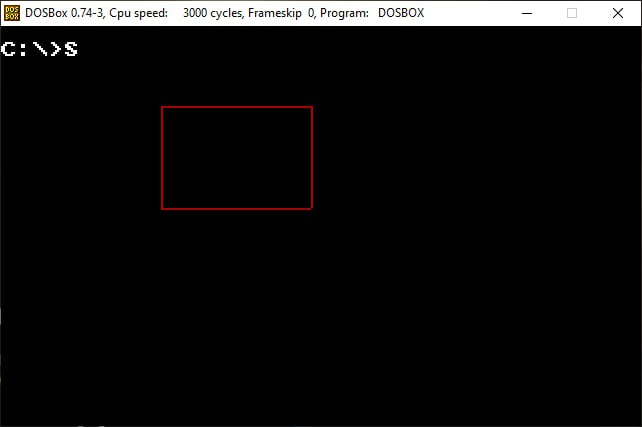
\includegraphics[width=0.90\textwidth]{rect.jpg}
    \caption{}
\end{figure}

\vspace{12pt}

\subsection*{Висновок} 
Я освоїв роботу з графікою використовуючи можливості BIOS на 16-бітному асембері.


\end{document}